
\documentclass[useAMS,usenatbib]{mn2e}
%\documentclass[usenatbib]{mn2e}
\usepackage{graphicx}
%\usepackage[nottoc]{tocbibind}
\setlength{\topmargin}{-1.2cm}

% If your system does not have the AMS fonts version 2.0 installed, then
% remove the useAMS option.
%
% useAMS allows you to obtain upright Greek characters.
% e.g. \umu, \upi etc.  See the section on "Upright Greek characters" in
% this guide for further information.
%
% If you are using AMS 2.0 fonts, bold math letters/symbols are available
% at a larger range of sizes for NFSS release 1 and 2 (using \boldmath or
% preferably \bmath).
%
% The usenatbib command allows the use of Patrick Daly's natbib.sty for
% cross-referencing.
%
% If you wish to typeset the paper in Times font (if you do not have the
% PostScript Type 1 Computer Modern fonts you will need to do this to get
% smoother fonts in a PDF file) then uncomment the next line
% \usepackage{Times}

%%%%% AUTHORS - PLACE YOUR OWN MACROS HERE %%%%%

% Journal definitions
\newcommand{\apj}[1]{ApJ}
\newcommand{\mnras}[1]{MNRAS}
\newcommand{\apjl}[1]{ApJL}
\newcommand{\pasj}[1]{PASJ}
\newcommand{\aj}[1]{AJ}
\newcommand{\nat}[1]{Nature}
\newcommand{\aap}{A\&A}

%%%%%%%%%%%%%%%%%%%%%%%%%%%%%%%%%%%%%%%%%%%%%%%%

\title[Beware the Effect of Edge-on Disks]{Gravitational Lens Modelling of Flux Ratio Anomalous System B1555+375}
\author[Hsueh et al.]{Jen-Wei Hsueh$^{1}$\thanks{E-mail:
email@address (AVR); otheremail@otheraddress (ANO)} and A. N.
Other$^{2}$\\
$^{1}$Physics Dept., University of California, Davis, 1 Shields Ave.
Davis, CA 95616, USA\\
$^{2}$Building, Institute, Street Address, City, Code, Country}
\begin{document}

%\date{Accepted 1988 December 15. Received 1988 December 14; in original form 1988 October 11}

\pagerange{\pageref{firstpage}--\pageref{lastpage}} \pubyear{2015}

\maketitle

\label{firstpage}

\begin{abstract}

Gravitational lens flux-ratio anomalies provide a powerful technique
for detecting the presence of dark matter substructure in distant
galaxies.  However, before using the statistics of systems with these
anomalies, it is imperative to ascertain that a given system does not
have properties that could plausibly cause the observed anomaly
without the need for substructure.  In this letter, we present the
case of the B1555+375 lens system, which has a strong radio-wavelength
flux-ratio anomaly but where the lensing galaxy is also revealed in
high-resolution imaging to have a clear edge-on disk component.  The
disk crosses directly over the pair of images that exhibit the
anomaly, and we show that simple models that include the disk can
reproduce the anomaly without requiring substructure.  
Other lens systems that we have observed with adaptive optics imaging
as part of the Strong lensing at High Angular Resolution Programme (SHARP)
show a similar behaviour and will be the subject of a future paper.  
These results suggest that the assumption that
all flux-ratio anomalies are due to substructure will likely overestimate
the substructure fraction in massive galaxies.

\end{abstract}

\begin{keywords}
gravitational lensing
\end{keywords}

\section{Introduction}

A common feature of simulations of structure formation is the presence
of thousands of subhaloes that are associated with larger mass haloes \citep[e.g.][]{Springel08}.
However, observations of the Local Group find many fewer satellite
galaxies than are predicted by the simulations, even when taking into
account completeness corrections arising from the limited sky coverage
imposed by the Galactic Plane and the latest discovery of new dwarf galaxies \citep{DES15,Kop15}.  
This is the famous ``missing satellite'' problem \citep{Klypin1999, Moore1999, S07}. In order to
understand this discrepancy, it is imperative to build up a large
sample of satellites/subhaloes in galaxies outside the Local Group.
 However, this process is challenging due to the faintness of the satellite
galaxies.  Furthermore, lower-mass satellites may not be able to
retain the gas needed for ongoing star formation \citep[e.g.,][]{P11},
rendering them effectively dark.  These factors make gravitational
lensing a powerful and promising tool for the detection of
substructure.

It was first suggested by \citet{Mao1998} that flux ratio anomalies observed in radio loud multiple images of lensed quasar could be interpreted as the telltale of the presence of substructure in lens galaxies.
Indeed, small perturbations in the gravitational potential are
sufficient to bring flux ratio anomalies in strong lensed systems \citep{Bradac02}. 
Moreover, unlike in the optical or infrared, in the radio band, lensed
images are not sensitive to micro lensing from stars nor dust
extinction. This makes flux ratio anomalies a promising tool to
detect dark matter substructures \citep{Dalal2002, N13}.  At present,
the amount of substructure derived from flux ratio anomalies is in
disagreement with predictions from numerical simulations, with the
former requiring a larger fraction of mass in substructure than
expected \citep{Xu14}. While this could be the result of small sample
statistics, it could also be the indication that flux ratio anomalies
have a different origin than substructure. 
%
An alternative method for
the detection of substructure in gravitational lens galaxies based on
the surface brightness distribution of extended arcs and Einstein rings
has been introduced by \citet{K05} and \citet{V09}. Interestingly, the fraction of
substructure measured with this \emph{gravitational imaging technique}
is currently in agreement with theoretical expectations \citep{V14a}.

While future large-scale surveys, such as the LSST, are expected to
deliver new large samples of gravitationally lensed quasars, in the
near future the discovery of new systems using narrow-line quasar
emission \citep{N14} will provide new invaluable statistical
perspective on current constraints based on flux ratio anomalies.  In
this letter, we explore the idea that not all flux ratio anomalies are
related to the presence of substructure, but that some originate in a
more complex lens galaxy mass distribution than initially
considered. To this end we use new infra-red data from the Strong
lensing at High Angular Resolution Program (SHARP; Fassnacht et al.,
in prep). The main goal of the SHARP project is to re-observe known
quadruple and Einstein ring lens systems at a much higher angular
resolution by making use of observations with (1) adaptive optics (AO)
on the Keck telescopes, (2) the Hubble Space Telescope, and (3) large
interferometric arrays \citep{SHARP12,V12}. In particular, to better
understand the causes of flux ratio anomalies in gravitational lenses
we focus on the B1555+375 lens system\citep{Marlow99}.  This system was
discovered in the Cosmic Lens All-Sky Survey \citep{CLASS1,CLASS2} and
has a pair of merging images that show a strong flux ratio anomaly at
radio wavelengths.  Follow-up observations ruled out radio propagation
effects as the cause of the anomaly \citep{K03,KD04}.  The B1555+375
system was included in both the observational and theoretical analysis
of \citet{Dalal2002} and \citet{Xu14} and, thus, understanding its
mass distribution is of key importance.  Our analysis makes use of
the new information obtained from the latest SHARP infrared imaging.
The paper is organized as follows: the latest SHARP data are
introduced in section 2; in section 3 we present the lens model while
the results of this analysis and their implications are discussed in
section 4.

\section{Data Collection \& Reduction}

\begin{figure*}
%\begin{minipage}{140mm}
%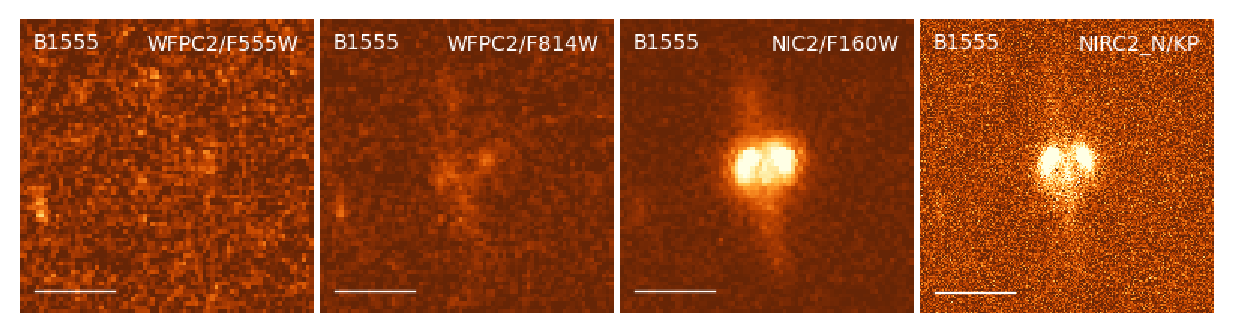
\includegraphics[width=140mm]{B1555_gallery.eps}
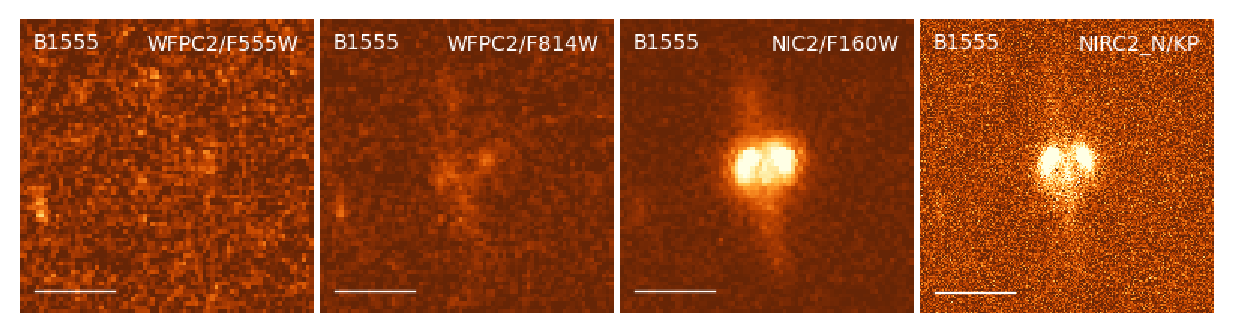
\includegraphics[width=0.95\textwidth]{B1555_gallery.eps}
\caption{High-resolution multiband imaging of the B1555+375 lens system.
All of the panels are 3\farcs7 on a side, and for each panel the scale bar 
represents 1\arcsec.  From left to right the figures show data from
HST/WFPC2 in the F555W band, HST/WFPC2 in the F814W band, HST/NICMOS/NIC2
in the F160W band, and Keck AO imaging in the $K^\prime$ band.
\label{fig:multiband}}
%
%\end{minipage}

\end{figure*}

\subsection{Keck Adaptive Optics Imaging}

The B1555+375 system was observed using the NIRC2 camera on the Keck 2
Telescope on the night of 2012 May 16 UT.  The adaptive optics system
was used, with the corrections derived from the laser guide star and a
$R$=14.4 tip-tilt that was located 45$^{\prime\prime}$ from the lens
system.  The ``narrow camera'' mode was used, giving a field of view
of roughly 10$^{\prime\prime}$\ on a side and a pixel scale of 10~mas.
Six dithered 300~s exposures were obtained in $K^{\prime}$ band.  The
data were reduced with the standard SHARP pipeline, which is a
python-based package that is a refinement of the process described in
\citet{Auger_EELS1}.  A cutout of the final reduced image is shown in
Fig.~\ref{fig:multiband} and again in Fig.~\ref{fig:merlin} with
contours from the MERLIN radio observations of \citet{Marlow99}
overlaid.  There are several notable features in the Keck AO data.
These include the nearly complete lack of emission associated with the
B and D lensed images, as can be seen by comparing the radio contours
to the $K^\prime$-band emission, and faint but clearly visible
emission from what appears to be an edge-on lensing galaxy.

\subsection{Hubble Space Telescope Archival Imaging}

The B1555+375 system was also observed by the Hubble Space Telescope
(HST) in three broad bands.  The optical data were obtained with the
Wide-Field Planetary Camera 2 (WFPC2) in the F555W and F814W bands
(GO-8804; PI: E.\ Falco), while the Near Infrared Multi-Object
Spectrograph (NICMOS) was used to observe the system in the $F160W$
band (GO-9744; PI: C.\ Kochanek).  The NICMOS observations were
obtained with the NIC2 camera.  We reduced all of the archival HST
data with the standard {\tt multidrizzle} pipeline [?? CHECK WITH
  MATT], producing final drizzled images with pixel scales of 50~mas.
The reduced images are shown in Figure~\ref{fig:multiband}.  The lens
system is not detected at high significance in the optical bands, but
is clearly seen in the NICMOS $F160W$ image.  The edge-on lensing
galaxy stands out in the NICMOS image.

The observation details of Keck AO and HST imaging are shown in Table 1.

\begin{table}
 \centering
 %\begin{minipage}{140mm}
  \caption{Multiband observation details of the B1555+375 lens system.}
  \begin{tabular}{@{}llccc}
  
\hline
  Telescope     &      Camera     &  Band & Date &$t_{exp}$ (s) \\

 \hline
   HST				&		WFPC2    &  F555W		&	2000/10/09 	&	5200\\
   HST				&		WFPC2    &  F814W		&	2000/10/09 &	5200\\
   HST				&		NICMOS/NIC2	&	F160W	&	2003/11/02 & 5376\\
   Keck2			&		NIRC2 AO	&   $K^\prime$	& 2012/05/16	&  1800\\
   \hline
\end{tabular}
%\end{minipage}
\end{table}

%===========================================================================

\section{Lens Modelling}

To model B1555+375, we use the lens modeling code {\tt glafic}
\citep{Oguri}.  The inputs to the model are the observed image
positions and flux densities measured by the radio observations of
\citet{Marlow99}.  These authors present a singular isothermal ellipsoid
(SIE) model that provides the first fit to the image positions but
does not reproduce the strong flux ratio anomaly between components A
and B.  \citep[see Fig.~6 and Tables 2 \& 3 in][]{Marlow99}.  Although
the flux ratio anomaly that is observed in the radio data may be
caused by substructure in the lensing galaxy, our high-resolution near
infrared imaging suggests another explanation.  In both the $K^\prime$
band adaptive optics data and the HST imaging (two rightmost panels in
Fig. 1), the lensing galaxy has a clear edge-on disk component with a
position angle of $\approx 10$ degree.  We therefore model the system
with a disk component in order to see if such a model can explain the
flux ratio anomaly without the need for substructure.  The edge-on
disk may also explain the system morphology that is observed in the
near infrared imaging.  In particular, neither image B nor image D is
detected in the Keck AO data (Fig.~\ref{fig:merlin}), and both of
these lensed images lie on or close to the edge-on disk.  Thus, strong
extinction in the disk could cause the lack of detection of these
images.

As a first trail of modelling, we create a single SIE model to 
justify the performance of a simple lensing potential. Consistent with previous studies
\citep{Marlow99, Xu14}, our single elliptical potential model cannot predict flux anomaly in B1555+375. 
We then create two separate models of the lensing potential.  In the
first we treat the lens as a SIE bulge and an exponential edge-on disk
(SIE+expdisk).  In the second model the disk is represented as a very
elongated SIE component (2-SIE).  The lens system is red, with a
strong jump in flux between the F814W (roughly I) and F160W (roughly
H) bands (Fig.~\ref{fig:multiband}), so we assign a lens redshift of
$z_\ell = 1.0$ and a source redshift of $z_s =1.5$. Our steps to explore the parameter space are: (1) Apply strong priors from SHARP AO image to the edge-on disk position angle and ellipticity, and use the best-fit model of \citet{Marlow99} as the start point of the bulge component and the source position. (2) Let all parameters without priors vary to reach a temporary best-fit. (3) Start with the best-fit in step 2 and let all parameters with priors vary to reach another best-fit (also ensure this best-fit is not far from the priors). (4) Let all parameters vary to reach the final optimal model. 
The full best-fit parameters are shown in Table
2. Both of these models predict fairly matched results with the radio
observation, and the 2-SIE model has a better performance in flux
ratios. The comparison of observation and our lens modelling is given
in Figure 3 and Tables 3 \& 4.
{\bf We have not included an external shear component into our model because the constraints provided by the image positions and  fluxes would not be sufficient 
to constrain such a model. However, we note that the image not affected by dust (image C) in the Keck AO data is consistent with negligible shear (i.e. shear strength $\Gamma_s=0.002$), when modelled with the pixelized technique by \citet{V09}.}

\begin{figure}
%\plotone{1555_ao_merlin_overlay.eps}
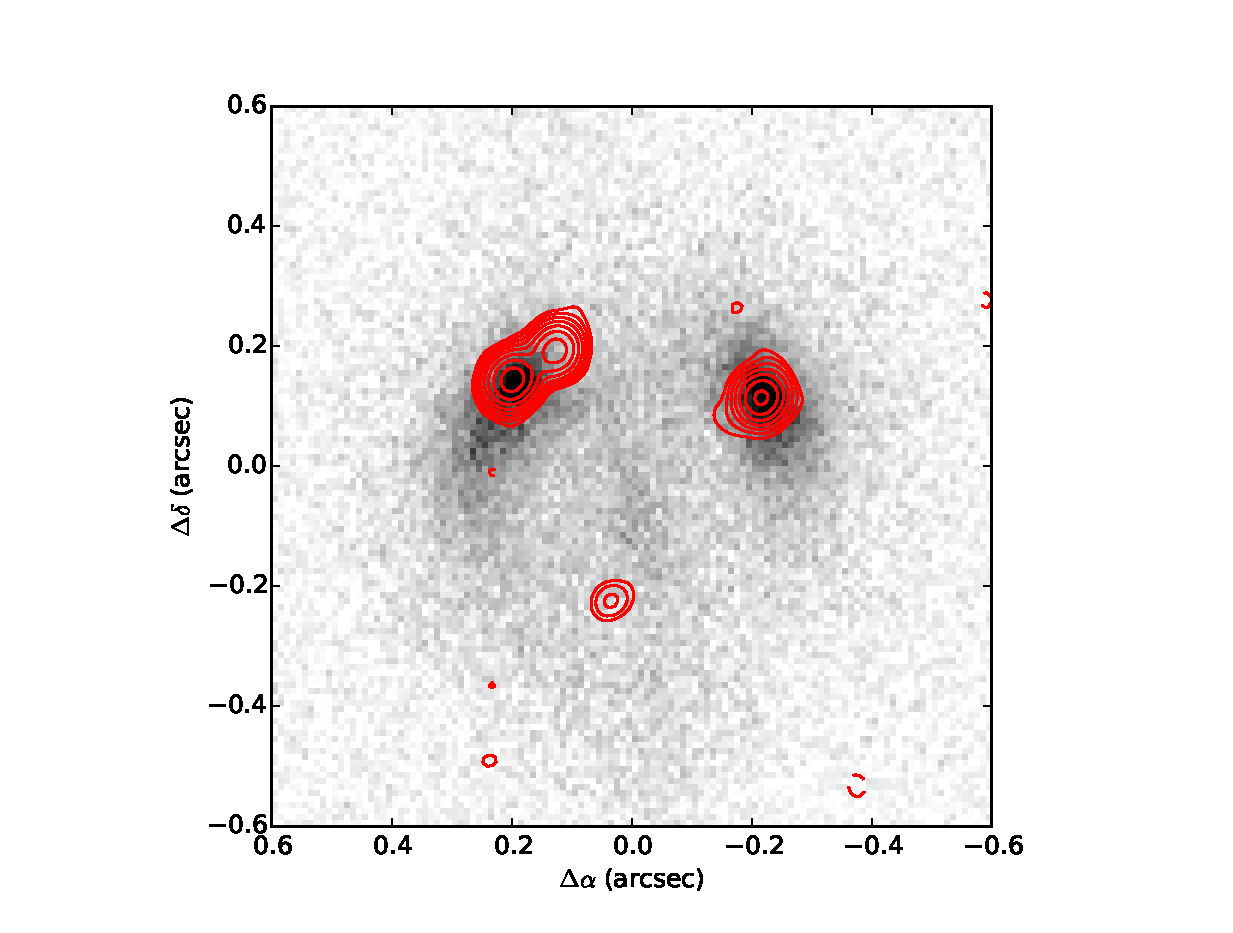
\includegraphics[width=84mm]{1555_ao_merlin_overlay.eps}
\caption{High-resolution  $K^\prime$ band imaging of the B1555+375 lens system 
with contours from the MERLIN observation of \citet{Marlow99} overlaid.
%
\label{fig:merlin}}
\end{figure}


\begin{figure}
%\plotone{point_source.eps}
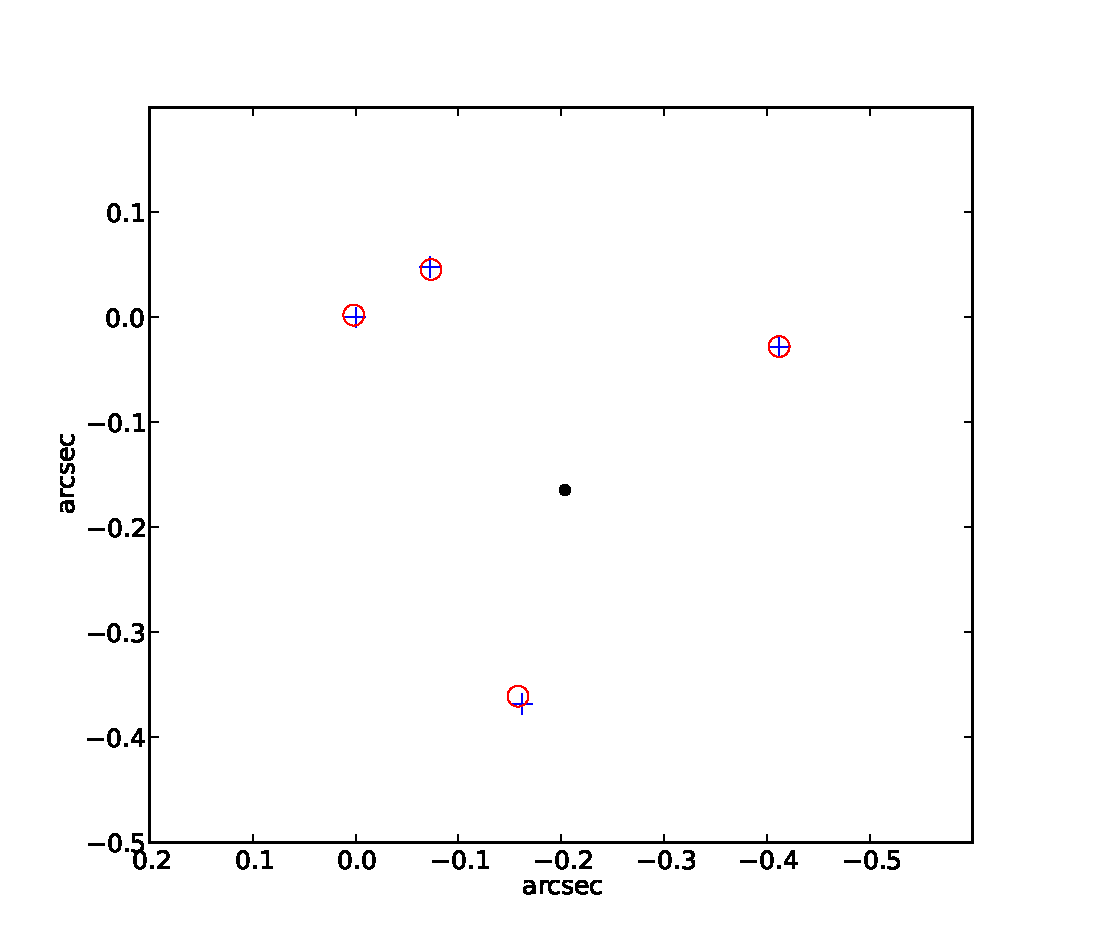
\includegraphics[width=84mm]{point_source.eps}
\caption{Radio observation(red open circle) and model-predicted(blue plus sign) image positions of B1555+375. The position of the source is at $(-0.2066,-0.1634)$ for SIE+Expdisk model, marked by a black filled circle. From left to right, four components are A, B (merging doubles), D(lowest spot), and C(right).\label{fig2}}
\end{figure}



\begin{table}
% \centering
% \begin{minipage}{140mm}
  \caption{Best-fit parameters of B1555+375 lens models.}
  \begin{tabular}{@{}ccc}
\hline 
 Parameter  & \multicolumn{2}{c}{Lens model} \\
		&SIE+expdisk& 2-SIE		   
\\
\hline
$x_1$  	  & $-0.1883$	& $-0.1813$  \\
$y_1$	  &$-0.1923$	&$-0.1695$  \\
$x_2$	  &$-0.1615$ 	&$-0.1593$  \\
$y_2$	  &$-0.2502$	& $-0.1843$  \\
$\sigma_1$ &$141.3$     & $144.9$ \\
$e_1$	  & $0.27$	& $0.27$ \\
$\theta_1$ &$105.5 \degr$ & $97.7 \degr$ \\
$M_{tot,2}$  & $3.59\times 10^{10} $  & ...	 \\  
$\sigma_2$ & ...        &$123.5$ \\  
$e_2$	  &$0.84$	&$0.83$  \\
$\theta_2$ &$7.4\degr$ &$7.4\degr$  \\
$r_e$	  & $0.20 ''$ &  ... \\
\hline
$\chi ^2$ & $1.05$ & $0.04$ \\
\hline
\end{tabular}

%\end{minipage}
\medskip
Subscripts 1 and 2 represent bulge and disk components in each model respectively. Positions are offsets from radio image component A measured in units of arcsec. The velocity dispersion $\sigma$ is in units of $km/s$ and disk mass $M_{tot}$ is in units of $h^{-1} M_{\odot}$. $e$ is ellipticity and $\theta$ is the position angle measured east of north.

\end{table}

\begin{table*}
%\centering
 \begin{minipage}{140mm}
  \caption{Radio observation and model-predicted lensed image positions.}
  \begin{tabular}{@{}ccccccc}

\hline

Component	&\multicolumn{2}{c}{MERLIN} 	 & \multicolumn{4}{c}{Model} \\
					&\multicolumn{2}{c}{5 GHz}		&	\multicolumn{2}{c}{SIE+expdisk} &\multicolumn{2}{c}{ 2-SIE}		\\
					 &East &North &East 		&North &East 		&North\\ 
\hline
A ........ &$0$    		&$0$		&$0.0000$ &$0.0000$   &   $0.0000$   &  $ 0.0000$\\  
B ........ &$-0.0726$ 	&$+0.0480$	&$-0.0726$ &$+0.0479$ & $-0.0726 $  &  $+0.0481$  \\  
C ........ &$-0.4117$  &$-0.0280$	&$-0.4117$ &$-0.0280$  & $-0.4117 $  &   $+0.0280$ \\  
D ........ &$-0.1619$  &$-0.3680$	&$-0.1610$ &$-0.3678$  & $-0.1620$    &  $+0.3682$ \\  
\hline
\end{tabular}

\end{minipage}
\medskip

Comparison between radio and model-predicted lensed image positions. Observation data quoted from Table 2 in \citet{Marlow99}. Position offsets are in unit of arcsec. Both SIE+expdisk and 2-SIE lens model-predicted positions well match to the radio observation.

\end{table*}

\begin{table}
% \centering
% \begin{minipage}{140mm}
  \caption{Flux ratios of B1555+375 components.}
  \begin{tabular}{@{}ccccccc}

\hline
	& MERLIN & VLA & \multicolumn{3}{l}{Model}\\
		&5 GHz & 15 GHz  & 1-SIE & SIE+expdisk & 2-SIE\\
\hline
$f_A/f_B$			&$1.75$ & $1.78$ &$1.07$& $1.66$ & $1.75$ \\ 
$f_A/f_C$		&$2.05$ 	&$2.37$ &$2.95$ & $1.33$ & $2.16$\\
$f_A/f_D$		&$13.08$ &$ 12.86$ &$2.00$& $5.83$ & $7.96$\\

\hline
\end{tabular}

%\end{minipage}
\medskip
Comparision between radio data and model-predicted flux ratios. The radio observation data is quoted from Tables 2 and Table 3 in \citet{Marlow99}. 1-SIE model is quoted from Tabel 5 in \citet{Marlow99}.

\end{table}

\section{Discussion}

Gravitational lensing is,  at present, the most powerful tool for
studying substructure in galaxies outside of the Local Universe, and
the flux ratio anomaly systems are a key aspect of these
investigations.  However, before using the flux ratio anomaly in any
given system to investigate structure formation and the properties of
dark matter, it is critical to eliminate other possible explanations
for the difference between the observed and expected fluxes, such as propagation effects and assumptions on the mass distribution of the lens galaxy.  
It is for this reason that much of the effort in the flux-ratio technique
has been focused on radio-loud lens systems.  At these wavelengths,
dust extinction and microlensing effects should be minimal
\citep[although see][for a rare example of radio microlensing]{K2000}.
Radio propagation effects can affect radio fluxes, as is clearly shown
in the B0128+437 system \citep{B04}.  However, these propagation
effects can be disentangled from substructure lensing because they
have well known dependencies on wavelength. \citet{KD04} examine all
eight radio loud flux anomalous lenses besides B0128+437, namely: MG
0414+0534, B0712+472, B1359+154, B1422+231, B1555+375, B1608+656,
B1933+503, and B2045+265.  They found no strong wavelength dependence
in the flux ratios of all these systems and therefore rule out radio
propagation effects as significant contributors to the observed
anomalies.

{\bf In this letter, we focus on the effect of more complicated mass distributions for the lens galaxy on flux ratio anomalies.
Traditionally, flux anomalous lensed quasars are radio loud systems that are firstly discovered in radio observations. While radio data provide reliable information on the positions and the fluxes of the lensed images, they are often unable to detect the lens galaxies. Moreover, lens modelling based only on the positions of the four images can be highly degenerate and prior assumptions play a key role in the interpretation of the observed flux ratio anomaly.
Since lens galaxies are mostly located at low redshift, optical and near-infrared observations are ideal to measure the light distribution of lens galaxies and obtain useful prior information  
on the underlying mass distribution. Indeed \citet{SHARP12} has shown that high resolution IR imaging can help to significantly improve the precision of the lens modelling. This improvement is even more dramatic in the case of B1555+375, where HST and SHARP AO high resolution imaging, has allowed us to detect, for the fist time, the presence of an edge-on disk. This new discovered edge-on disk provides a strong prior for our lens modelling.  With a bulge plus an edge-on disk, our models produce matches to both the radio image
positions and their flux ratio, while models with only one SIE component \citep{Marlow99,Xu14} fail to reproduce the fluxes correctly. Our successful modelling indicates that the
kiloparsec-scale structure of the lens galaxy itself is sufficient to explain the flux ratio anomalies in B1555+375, without any need to invoke the presence of substructure.  }

From a theoretical perspective, \citet{Xu14} find that substructures
cannot explain the observed radio flux anomalies in all the lenses
that were considered. By adding subhaloes from numerical simulations
on to these systems, only one out of eight radio loud systems
reproduces the level of flux anomalies seen in the data.  The rest of
them are unlikely (only $1 \% - 4 \%$ probability) to have flux
anomalies produced by substructure, including our target B1555+375.
In fact, among those eight radio lenses, B1555+375 is one of the most
anomalous systems, but it is also one of the most challenging systems
to explain by substructures. \citet{Xu14} have concluded that the failure in
predicting flux ratios is most likely due to oversimplified/improper lens
modelling. They also point out that the SIE component and the external
shear in their model are orthogonal, indicating a possible missing
ingredient in the lens model. Their results are consistent with the SHARP
$K^{\prime}$ band observations, in which an edge-on disk crosses the
radio merging double and which fully accounts for the observed flux ratio anomaly.  In general, it is well known 
\citep[e.g,][]{Ka91} that lens models based only on the locations of lensed
quasar/AGN images have large degeneracies. Therefore, before
concluding that the flux ratios in any given lens system are a result
of substructure, it is critical to explore a range of smooth models
that are informed by additional observations or to do a comprehensive
analysis such as that conducted by \citet{Xu14}. Otherwise, derived
substructure fractions should be considered as upper limits.
 
%Although the number of radio loud flux anomalous lensed
%quasars remains small, a new technique using narrow-line emission
%regions will enlarge the sample and bring statistical perspective on
%substructures in the near future \citep{N14}. 

\section{Conclusions}
{\bf In this letter we have taken advantage of the power of multi-wavelength high resolution data to investigate whether flux ratio anomalies could be explained by more complex smooth models for the lens galaxy mass distribution rather than substructure. Thanks to new imaging from the SHARP $K^{\prime}$ band observations of the gravitational lens system B1555+375, we have identified the existence of a previously undetected edge-on disk. By including this disk in the mass model of the lens galaxy, we find a good fit for both the positions and flux ratios of the lensed images. Our results clearly demonstrate that the lack of knowledge on the lens galaxy mass distribution, combined with the limited information provided by the position of a few lensed images, can lead to improper lens models and a misinterpretation of the origin of flux ratio anomalies. 
We stress, therefore, that one should be very careful when interpreting the nature of flux ratio anomalies, as prior assumptions on the lens mass distribution are a significant source of bias. Our analysis shows that in order to derive precise quantification of the substructure population and any derived properties from strongly lensed flux anomalous systems, it is crucial to have a careful estimation of non-substructure effects. In fact, even in the presence of mass substructures, the observed flux ratio anomalies could be still dominated by the complex structure of the lens galaxy. Finally, additional near-infrared AO imaging from SHARP shows that B1555+375 is not the only system having a significant disk component detection in
the lensing galaxy.  These systems will be investigated in future work, but the images alone strongly suggest that other lens systems have similar links between flux-ratio anomalies and disk components. 
}

%. Modelling with only four image positions from radio data can also cause a lot of degeneracy. With the first system analyzing and finding an edge-on disk originated flux ratio anomaly, our follow up will be explore other similar SHARP systems. In Figure 3, all of these systems have a recognizable edge-on disk in infrared imaging. An edge-on disk structure may also be able to explain the flux ratio anomalies of these systems.
 %From the successful modelling of B1555+375,  we expect more flux anomalous systems requiring complex lens models (e.g. include an exponential disk), rather than just assuming smooth potential. Although the number of radio loud flux anomalous lensed quasars remains small, a new technique using narrow-line emissions will enlarge the sample and bring statistical perspective on substructures in the near future \citep{N14}. If the non-substructure effect from edge-on disks does not included, expected ``false'' substructure detections can serverly bias the data analysis. 
% This breaks the idea that in strongly lensed quasars, radio flux ratio
% anomalies are most likely originated from substructure
% perturbations. Our discovery shows a complex lens galaxy mass
% distribution can dominate flux ratio anomalous phenomena in a strongly
% lensed system.
% We would like to draw attention to the possible impacts on
% substructure searching from this enge-on disk orginated flux
% anomalies. It is a sign that researchers should be careful about the
% flux anomalies fraction in lensed quasars. It may be worth considering
% an upper limit of flux anomalies fraciton from observation results to
% avoid over estimate the number of substructure detections. For further
% analysis on substurcture population, mass function etc., it is always
% important to rule out other non-substructure effects.

\section*{Acknowledgments}
S.V. is grateful to Dandan Xu for useful discussion on the nature of flux ratio anomalies in high resolution numerical simulations.
\bibliographystyle{mn2e}
\bibliography{reference.bib}




\label{lastpage}

\end{document}
